\documentclass{article}
\usepackage[margin=1in]{geometry}
\usepackage[english]{babel}
\usepackage{amsmath, amssymb, amstext, tikz, tikz-qtree, kbordermatrix}
\usetikzlibrary{calc,shapes.multipart,chains,arrows}
\linespread{1.5}
\parindent=0in

\tikzset{edge from parent/.append style={->}}

\begin{document}
\textbf{\textit{22.1-2}}\\
Give an adjacency-list representation for a complete binary tree on 7 vertices. Give
an equivalent adjacency-matrix representation. Assume that vertices are numbered
from 1 to 7 as in a binary heap.\\

We let $G$ be a complete binary tree on 7 vertices such that it is a heap. Then, we assume the graph to look roughly as so,
\begin{center}
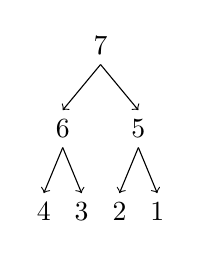
\begin{tikzpicture}
\Tree[.7 
		[.6 
			[.4 ]
            [.3 ]]
		[.5 
			[.2 ]
         	[.1 ]]]
\end{tikzpicture}
\end{center}

Then, we can represent $G = (V, E)$ as a series of adjacency-lists. The adjacency-lists are as so,
\begin{center}
%7 adjacency list
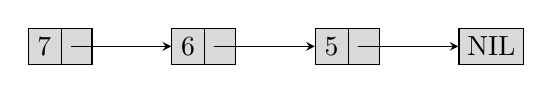
\begin{tikzpicture}[list/.style={rectangle split, rectangle split parts=2,
    draw, rectangle split horizontal}, >=stealth, start chain]
  \node[list,on chain, fill = black!15] (a) {7};
  \node[list,on chain, fill = black!15] (b) {6};
  \node[list,on chain, fill = black!15] (c) {5};
  \node[on chain,draw,inner sep=3pt, fill = black!15] (d) {NIL};
  \draw[->] let \p1 = (a.two), \p2 = (a.center) in (\x1,\y2) -- (b);
  \draw[->] let \p1 = (b.two), \p2 = (b.center) in (\x1,\y2) -- (c);
  \draw[->] let \p1 = (c.two), \p2 = (c.center) in (\x1,\y2) -- (d);
\end{tikzpicture}\\
%6 adjacency list
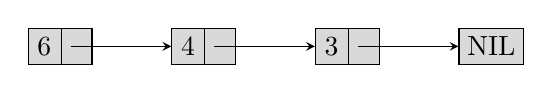
\begin{tikzpicture}[list/.style={rectangle split, rectangle split parts=2,
    draw, rectangle split horizontal}, >=stealth, start chain]
  \node[list,on chain, fill = black!15] (a) {6};
  \node[list,on chain, fill = black!15] (b) {4};
  \node[list,on chain, fill = black!15] (c) {3};
  \node[on chain,draw,inner sep=3pt, fill = black!15] (d) {NIL};
  \draw[->] let \p1 = (a.two), \p2 = (a.center) in (\x1,\y2) -- (b);
  \draw[->] let \p1 = (b.two), \p2 = (b.center) in (\x1,\y2) -- (c);
  \draw[->] let \p1 = (c.two), \p2 = (c.center) in (\x1,\y2) -- (d);
\end{tikzpicture}\\
%5 adjacency list
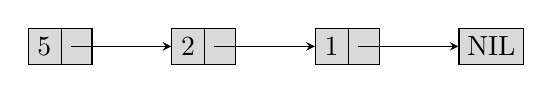
\begin{tikzpicture}[list/.style={rectangle split, rectangle split parts=2,
    draw, rectangle split horizontal}, >=stealth, start chain]
  \node[list,on chain, fill = black!15] (a) {5};
  \node[list,on chain, fill = black!15] (b) {2};
  \node[list,on chain, fill = black!15] (c) {1};
  \node[on chain,draw,inner sep=3pt, fill = black!15] (d) {NIL};
  \draw[->] let \p1 = (a.two), \p2 = (a.center) in (\x1,\y2) -- (b);
  \draw[->] let \p1 = (b.two), \p2 = (b.center) in (\x1,\y2) -- (c);
  \draw[->] let \p1 = (c.two), \p2 = (c.center) in (\x1,\y2) -- (d);
\end{tikzpicture}\\
%4 adjacency list
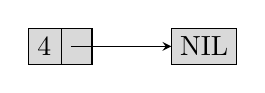
\begin{tikzpicture}[list/.style={rectangle split, rectangle split parts=2,
    draw, rectangle split horizontal}, >=stealth, start chain]
  \node[list,on chain, fill = black!15] (a) {4};
  \node[on chain,draw,inner sep=3pt, fill = black!15] (d) {NIL};
  \draw[->] let \p1 = (a.two), \p2 = (a.center) in (\x1,\y2) -- (d);
\end{tikzpicture}\\
%3 adjacency list
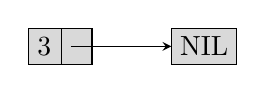
\begin{tikzpicture}[list/.style={rectangle split, rectangle split parts=2,
    draw, rectangle split horizontal}, >=stealth, start chain]
  \node[list,on chain, fill = black!15] (a) {3};
  \node[on chain,draw,inner sep=3pt, fill = black!15] (d) {NIL};
  \draw[->] let \p1 = (a.two), \p2 = (a.center) in (\x1,\y2) -- (d);
\end{tikzpicture}\\
%2 adjacency list
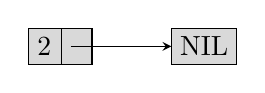
\begin{tikzpicture}[list/.style={rectangle split, rectangle split parts=2,
    draw, rectangle split horizontal}, >=stealth, start chain]
  \node[list,on chain, fill = black!15] (a) {2};
  \node[on chain,draw,inner sep=3pt, fill = black!15] (d) {NIL};
  \draw[->] let \p1 = (a.two), \p2 = (a.center) in (\x1,\y2) -- (d);
\end{tikzpicture}\\
%1 adjacency list
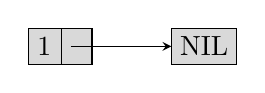
\begin{tikzpicture}[list/.style={rectangle split, rectangle split parts=2,
    draw, rectangle split horizontal}, >=stealth, start chain]
  \node[list,on chain, fill = black!15] (a) {1};
  \node[on chain,draw,inner sep=3pt, fill = black!15] (d) {NIL};
  \draw[->] let \p1 = (a.two), \p2 = (a.center) in (\x1,\y2) -- (d);
\end{tikzpicture}
\end{center}
We can also represent $G = (V, E)$ as an adjacency-matrix. Then, the adjacency-matrix is as so,

\[
  G = \quad \kbordermatrix{
    & 1 & 2 & 3 & 4 & 5 & 6 & 7\\
    1 & 0 & 0 & 0 & 0 & 0 & 0 & 0\\
    2 & 0 & 0 & 0 & 0 & 0 & 0 & 0\\
    3 & 0 & 0 & 0 & 0 & 0 & 0 & 0\\
    4 & 0 & 0 & 0 & 0 & 0 & 0 & 0\\
    5 & 1 & 1 & 0 & 0 & 0 & 0 & 0\\
    6 & 0 & 0 & 1 & 1 & 0 & 0 & 0\\
    7 & 0 & 0 & 0 & 0 & 1 & 1 & 0\\
  }
\]


\end{document}